\chapter{L"osung der W"armeleitungsgleichung}
\rhead{W"armeleitungsgleichung}

\chapterauthor{Andreas M"uller}

Die W"armeleitungsgleichung ist die prototypische parabolische
partielle Differentialgleichung.
In diesem Kapitel werden die Eigenheiten ihrer numerischen L"osung
diskutiert.

\section{Problemstellung}
\lhead{Problemstellung}
Die W"armeleitungsgleichung f"ur einen Stab
auf dem Interval $[0,1]$ ist die partielle Differentialgleichung
\begin{equation}
\frac{\partial u}{\partial t}=\frac{\partial^2 u}{\partial x^2}, \qquad
0<x<1,\;t>0.
\label{heat:pdgl}
\end{equation}
Der Stab soll an den Enden mit W"armereservoirs verbunden sein, die
die Temperatur an den Enden festlegen. Sie kann mit der Zeit varieren.
Dies wird ausgedr"uckt durch
Randbedingungen
\begin{align}
u(t,0)&=g_0(t),
&
u(t,0)&=g_1(t),&t&>0.
\label{heat:rand}
\end{align}
Die L"osung wird festgegelegt durch die Temperaturverteilung zu Beginn,
also durch
\begin{align}
u(0,x)=f(x),\qquad 0<x<1.
\end{align}
Gesucht ist ein numerisches L"osungsverfahren, welches die
W"armeleitungsgleichung numerisch l"ost.

Eine interessante und unphysikalische Eigenschaft der W"armeleitungsgleichung
ist die Existenz von L"osungen mit unendlich schneller Wirkungsausbreitung.
Die Funktion
\[
u(t,x)=\frac1{\sqrt{2t}}e^{-\frac{x^2}{4t}}
\]
hat die folgenden Ableitungen:
\begin{align*}
\frac{\partial u}{\partial x}&=
-
\frac{x}{t}
\frac1{\sqrt{2t}}
e^{-\frac{x^2}{4t}}
&
\frac{\partial^2 u}{\partial x^2}&=
\biggl(\frac{x^2}{4t^2}-\frac1{2t}\biggr)
\frac1{\sqrt{2t}}
e^{-\frac{x^2}{4t}}
\\
\frac{\partial u}{\partial t}&=
\biggl(\frac{x^2}{4t^2}-\frac1{2t}\biggr)
\frac1{\sqrt{2t}}
e^{-\frac{x^2}{4t}}
\end{align*}
Die Funktion $u$ ist also eine L"osung der W"armeleitungsgleichung
(\ref{heat:pdgl}).
F"ur $t\to 0$ strebt $u(t,x)$ gegen eine Dirac $\delta$-Funktion
im Punkt 0.
Dies bedeutet, dass W"arme, die zur Zeit $t=0$ nur im Punkte vorhanden
ist, unmittelbar danach f"ur alle $t$ in Form eines Wertes $u(t,x) > 0$
sp"urbar ist.
Die W"arme im Punkt $0$ hat sich also mit unendlich grosser Geschwindigkeit
ausgebreitet.

\section{Diskretisation\label{heat:section-diskretisation}}
\begin{figure}
\begin{center}
\includegraphics[width=0.70\hsize]{heat/heat-1.pdf}
\end{center}
\caption{Diskretisation der W"armeleitungsgleichung. 
Aus jeweils drei horizontal benachbarten Punkten k"onnen die zweiten
Ableitungen berechnet werden.
Zwei in $t$-Richtung benachbarte solche Werte ergeben einen Mittelwert,
der f"ur die zweite Ableitung im Punkt $(i+\frac12,j)$ (schwarz)
stehen kann. Die erste Ableitung nach $t$ in diese Punkt kann aus
dem Differenzenquotienten ermittelt werden. So entstehen lineare
Gleichungen, die jeweils drei benachbarte noch nicht bekannte
$u$-Werte (rot) mit bereits bekannten Werten (blau) vernk"upfen.
\label{heat:diskretisation1}}
\end{figure}
Zur Diskretisation w"ahlen wir im Gebiet $[0,1]\times \mathbb R_+$ ein
Gitter. 
Da $x$- und $t$-Richtung offensichtlich nicht symmetrisch sind,
lassen wir offen, welche Gitterkonstanten wir in diesen Richtungen
verwenden wollen, und nennen Sie $h_x=1/n$ und $h_t$. 
Die Funktion $u(t,x)$ wird jetzt ersetzt durch die Werte von $u$ auf
den Gitterpunkten, wir schreiben
\[
u_{ij} = u(ih_t, jh_x),\quad i\ge 0, 0\le j \le n.
\]
Durch die Randbedingungen wird ein Teil dieser Variablen bereits
festgelegt:
\begin{align*}
u_{0j}&=f(jh_x)&1&\le x < n\\
u_{i0}&=g_0(ih_t)&i&>0\\
u_{i1}&=g_1(ih_t)&i&>0\\
\end{align*}
Die Diskretisation der Differentialgleichung verwendet die in
Abschnitt~\ref{subsection-motivation} Methode verwenden.
Die zweite partielle Ableitung von $u$ nach $x$ im Punkt $(ih_t, jh_x)$ 
kann durch
\begin{equation}
\frac1{h_x^2}(u_{i,j-1}-2u_{ij}+u_{i,j+1})
\label{heat:2ableitung}
\end{equation}
approximiert werden.
F"ur die erste partielle Ableitung nach $t$ ist man versucht,
den Differenzenquotienten
\begin{equation}
\frac1{h_t}(u_{i+1,j}-u_{ij})
\label{heat:1ableitung}
\end{equation}
zu verwenden.
Dieser Differenzenquotient ist aber eher eine Approximation f"ur
$\partial u/\partial t$ im Punkt $((i+\frac12)h_t, jh_x)$,
nicht $(ih_t,jh_x)$, man kann ihn also nicht direkt mit der
Approximation (\ref{heat:2ableitung}) f"ur die zweite Ableitung
in Beziehung setzen.
Man kann aber durch Mittelwertbildung aus (\ref{heat:2ableitung}) f"ur
die Punkte $(ih_t, jh_x)$ und $((i+1)h_t, jh_x)$ einen N"aherungswert
f"ur die zweite Ableitung finden, der sich mit der Approximation
f"ur die ersten Ableitung (\ref{heat:1ableitung}) setzen l"asst,
n"amlich
\begin{align}
\frac12\biggl(
\frac1{h_x^2}(u_{i,j-1}-2u_{ij}+u_{i,j+1})
+
\frac1{h_x^2}(u_{i+1,j-1}-2u_{i+1,j}+u_{i+1,j+1})
\biggr)
&=
\frac1{h_t}(u_{i+1,j}-u_{ij})
\label{heat:diskret}
\end{align}
Wir stellen die Gleichung um so, dass der linken Seite nur die 
Variablen f"ur die Zeit $(i+1)h_t$ stehen, und rechts nur die
Varaiblen f"ur die Zeit $ih_t$:
\begin{align}
\frac1{2h_x^2}(u_{i+1,j-1}-2u_{i+1,j}+u_{i+1,j+1})-\frac1{h_t}u_{i+1,j}
&=
-\frac1{2h_x^2}(u_{i,j-1}-2u_{ij}+u_{i,j+1})-\frac1{h_t}u_{ij}
\notag
\\
\frac1{2h_x^2}u_{i+1,j-1}
-\biggl(\frac1{h_x^2}+\frac1{h_t}\biggr)u_{i+1,j}
+\frac1{2h_x^2} u_{i+1,j+1}
&=
-\frac1{2h_x^2}u_{i,j-1}
+\biggl(\frac1{h_x^2}-\frac1{h_t}\biggr)u_{ij}
-\frac1{2h_x^2} u_{i,j+1}
\label{heat:gleichung}
\end{align}
Dies ist ein lineare Gleichung f"ur die Variablen $u_{i+1,j}$.
Die rechte Seite wird berechnet aus den Werten von $u_{ij}$,
f"ur $i=0$ steht dazu die Anfangsfunktion $f$ zur Verf"ugung.

Das Gleichungssystem (\ref{heat:gleichung}) hat die Matrix
\begin{equation}
A=
\underbrace{
\frac1{2h_x^2}
\begin{pmatrix}
-2& 1& 0&      &  \\
 1&-2& 1&      &  \\
 0& 1&-2&      &  \\
  &  &  &\ddots&  \\
  &  &  &      &-2
\end{pmatrix}}_N
\underbrace{
-\frac1{h_t}
\begin{pmatrix}
 1& 0& 0&      &  \\
 0& 1& 0&      &  \\
 0& 0& 1&      &  \\
  &  &  &\ddots&  \\
  &  &  &      & 1
\end{pmatrix}}_M
=N + M.
\label{heat:zerlegung}
\end{equation}
Die Matrix ist tridiagonal, und l"asst sich effizient mit dem
Gauss-Algorithmus l"osen.
Dieser Vorteil verschwindet allerdings, sobald das Problem auf
mehr Dimensionen verallgemeinert wird.
Wir wollen daher diesen Ansatz nicht weiterverfolgen, und stattdessen
versuchen, ein iteratives L"osungsverfahren anzuwenden.

Die Matrix $A$ hat eine naheliegende Zerlegung $A=N+M$, so dass
die allgemeine Theorie angewendet werden kann "uber iterative Verfahren,
die zu zerlegbare Matrizen geh"oren.
Schreiben wir $u^{(k)}_{i+}=u^{(k)}_{i+1,j}$ f"ur die $k$-te Iteration f"ur die
L"osung $u_{i+1,j}$ der Gleichung (\ref{heat:gleichung}).
Die allgemeine Theorie besagt, dass der iterative Algorithmus mit
Iterationsformel
\begin{equation}
u^{(k)}_{i+1}=M^{-1}(b-Nu_{i+1}^{(k-1)}),\qquad b=Mu_{i}-Nu_{i},
\label{heat:iteration}
\end{equation}
konvergiert, wenn die Matrix $M^{-1}N$ Spektralradius kleiner als $1$ hat.
Im vorliegenden Fall ist $M=\frac1{h_t}E$ sehr einfach zu invertieren,
es ist $M^{-1}=h_tE$, so dass die fragliche Matrix 
\[
M^{-1}N=\frac{h_t}{2h_x^2}
\begin{pmatrix}
-2& 1& 0&      &  \\
 1&-2& 1&      &  \\
 0& 1&-2&      &  \\
  &  &  &\ddots&  \\
  &  &  &      &-2
\end{pmatrix}
=\frac{h_t}{2h_x^2}\operatorname{tridiag}_n(1,-2,1)
\]
ist.
Der Spektralradius ist
\[
\varrho(M^{-1}N)
=
\varrho\biggl(\frac{h_t}{2h_x^2}\operatorname{tridiag}_n(1,-2,1)\biggr)
=
\frac{h_t}{2h_x^2}\varrho(\operatorname{tridiag}_n(1,-2,1)),
\]
wir haben den folgenden Satz bewiesen:

\begin{satz}
Das Iterationsverfahren (\ref{heat:iteration}) konvergiert, wenn 
\[
\frac{h_t}{2h_x^2}\varrho(\operatorname{tridiag}_n(1,-2,1))<1.
\]
\end{satz}

Wir m"ussen also herausfinden, wie gross der Betrag des
betragsm"assig gr"ossten Eigenwerts
der tridiagonalen Matrix $\operatorname{tridiag}_n(1,-2,1)$ ist.
Diese Frage wird von folgendem Satz beantwortet.

\begin{satz}
\[
\varrho(\operatorname{tridiag}_n(1,-2,1))<4.
\]
\end{satz}

\begin{proof}[Beweis]
Wir berechnen das charakteristische Polynom und zeigen dann, dass es
keine Nullstellen mit Betrag $>4$ hat.
\begin{align*}
\chi_n(\lambda)
&=
\det(\operatorname{tridiag}_n(1,-2-\lambda,1)
=
\left|
\,
\begin{matrix}
-2-\lambda&         1&      &          \\
1         &-2-\lambda&      &          \\
          &          &\ddots&          \\
          &          &      &-2-\lambda
\end{matrix}
\,
\right|
\\
&=(-1)^n
\left|
\,
\begin{matrix}
2+\lambda&        -1&      &         \\
-1        &2+\lambda&      &         \\
          &         &\ddots&         \\
          &         &      &2+\lambda
\end{matrix}
\,
\right|
=(-1)^n p_n(2+\lambda)=(-1)^np_n(\mu)
\end{align*}
Das Polynom $p_n(\mu)$ kann mit dem Entwicklungssatz ermittelt
werden:
\begin{align}
p_n(\mu)
&=
\left|
\,
\begin{matrix}
\mu& -1&   &      &   \\
-1 &\mu& -1&      &   \\
   & -1&\mu&      &   \\
   &   &   &\ddots&   \\
   &   &   &      &\mu
\end{matrix}
\,
\right|
=
\mu
\left|
\,
\begin{matrix}
\mu& -1&      &   \\
 -1&\mu&      &   \\
   &   &\ddots&   \\
   &   &      &\mu
\end{matrix}
\,
\right|
-(
-1)\cdot
\left|
\,
\begin{matrix}
 -1&   &      &   \\
 -1&\mu&      &   \\
   &   &\ddots&   \\
   &   &      &\mu
\end{matrix}
\,
\right|
\notag
\\
&=\mu p_{n-1}(\mu)- p_{n-2}(\mu).
\label{heat:rekursion}
\end{align}
Wir haben also eine Rekursionsgleichung f"ur die Polynome $p_n(\mu)$.
Die Anfangsbedingungen der Rekursion sind
\begin{align*}
p_1(\mu)&=\mu,\\
p_2(\mu)&=\mu^2-1.
\end{align*}
Wir behaupten, dass $p_n(\mu)$ keine Nullstellen mit $|\mu|>2$ hat.
Zun"achst stellen wir fest, dass $|p_2(\mu)| > |p_1(\mu)|$ ist, solange
$|\mu| > 2$, wie man sich durch eine Zeichnung der Graphen von $p_1(\mu)$
und $p_2(\mu)$ "uberzeugen kann.
Wir wollen jetzt mit vollst"andiger Induktion zeigen,
dass ganz allgemein
\begin{equation}
|p_n(\mu)| > |p_{n-1}(\mu)|
\label{heat:pnminorization}
\end{equation}
f"ur alle Werte $|\mu|>2$ und alle $n>1$ gilt. Die Induktionsverankerung
haben wird soeben gegeben.

F"ur den Induktionsschritt d"urfen wir also annehmen,
dass $|p_n(\mu)| > |p_{n-1}(\mu)|$, und m"ussen zeigen,
dass auch $|p_{n+1}(\mu)| > |p_n(\mu)|$ gilt.
Aus der Rekursionsformel (\ref{heat:rekursion})
kann man jetzt folgern:
\begin{align*}
|p_{n+1}(\mu)|
&=|\mu p_{n}(\mu) - p_{n-1}(\mu)|\\
&\ge |\mu|\cdot |p_{n}(\mu)| - |p_{n-1}(\mu)|\\
&>  |\mu|\cdot |p_{n}(\mu)| - |p_{n}(\mu)|\\
&=(|\mu|-1) p_{n}(\mu) > p_{n}(\mu)
\end{align*}
wegen $|\mu|>2$.
Damit ist der Induktionsschritt vollzogen.

Aus (\ref{heat:pnminorization})
kann man aber auch ablesen, dass $p_n(\mu)$ keine Nullstellen
haben kann mit $|\mu| > 2$, jede Nullstellen von $p_n(\mu)$ muss daher
$|\mu|<2$ erf"ullen.

Uns interessieren nat"urlich die Eigenwerte, also die Werte $\lambda=\mu-2$,
f"ur die $p_n(\mu)=0$ ist. Es folgt
\[
|\lambda|=|\mu - 2| \le |\mu|+2 \le 4,
\]
also kann kein Eigenwert einen Betrag $>4$ haben, der Spektralradius ist $4$.
\end{proof}
\begin{satz}
\label{heat:satz-konvergenz}
Das Iterationsverfahren (\ref{heat:iteration}) konvergiert, wenn 
\[
\frac{2h_t}{h_x^2}<1
\qquad
\Leftrightarrow
\qquad
h_t<\frac{h_x^2}2.
\]
\end{satz}
Halbiert man die Gitterkonstante $h_x$ in $x$-Richtung, dann muss man
die Zeitschritte viermal kleiner machen, damit das Verfahren immer
noch konvergent ist.

Die allgemeine Theorie l"asst noch etwas genauere Aussagen "uber die
Konvergenzgeschwindigkeit.
Der Fehler nach $k$ Iterationsschritten ist $|\varrho(M^{-1}N)|^k$.
Wenn die Konvergenz einigermassen schnell sein soll, dann muss
der Spektralradius klein gemacht werden.
Die Anzahl $k$ der Iterationsschritte, um Genauigkeit $\varepsilon< 1$ zu
erreichen ist
\[
k\ge
\log\varepsilon
\log\biggl(\frac{2h_t}{h_x^2}\biggr)^{-1}.
\]

Halbiert man $h_t$, dann wird in jedem Iterationsschritt ein zus"atzliches
Bit Genauigkeit gewonnen.
Wenn man mit der Schrittweite $h_t$ die verlangte Genauigkeit
von 32bit in 32 Schritten erreicht, dann kann man mit
Schrittweite $h_t/2$ diese Genauigkeit in 16 Schritten erreichen.
Nat"urlich muss man jetzt
zwei $h_t$-Schritte durchf"uhren, man hat also nichts gewonnen.

Satz \ref{heat:satz-konvergenz} zeigt, dass mit steigender Aufl"osung
in der Ortskoordinate die Aufl"osung in der Zeitkoordinate "uberprpoprtional
gesteigert werden muss.
Dies ist der numerische Ausdruck daf"ur, dass die W"armeleitungsgleichung
unendlich schnelle Wirkungsausbreitung modelliert.

\section{Parallelisierungsansatz}
Die numerische L"osung des diskretisierten Problems soll jetzt parallelisiert
werden.
Im Abschnitt~\ref{heat:section-diskretisation} wurde dargelegt, dass 
die Werte $u_{ij}$ jeweils nur f"ur einen Wert von $i$ berechnet
werden k"onnen.
Erst wenn die $u_{ij}$ berechnet sind kann man weitergehen und die
$u_{i+1,j}$ berechnen.
Die einzige Parallelisierungsm"oglichkeit steckt also in den der Berechnung
von $u_{ij}$ aus $u_{i-1,j}$ mit Hilfe des Iterationsverfahrens
(\ref{heat:iteration}).

Innerhalb des Iterationsverfahrens ist die einzige
Parallelisierungsm"oglichkeit wieder nur die Anwendung von
(\ref{heat:iteration}).
Die Parallelisierung muss daher den Definitionsbereich in einzelne
Intervalle $J_r=\{j_r,j_r+1,\dots,j_{r+1}-1\}$ von Indizes aufteilen,
in denen die Iteration durchgef"uhrt werden kann. 
F"ur den Wert von $u_{i,j}^{(k)}$ werden die Werte
$u_{i-1,j-1}^{(k-1)}$, $u_{i-1,j}^{(k-1)}$ und $u_{i-1,j+1}^{(k-1)}$ ben"otigt. 
F"ur die inneren Punkte im Interval $J_r$, als $j_r < j < j_{r+1}-1$
sind also alle ben"otigten Indizes in $J_r$, aber f"ur die
Werte $u_{ij_r}$ und $u_{i,j_{r+1}-1}$ sind zus"atzlich Indizes
aus den benachbarten Intervallen $J_{r-1}$ und $J_{r+1}$ n"otig.

Parallelisiert man den Algorithmus mit Hilfe von OpenMPI, reicht es also
nicht, dass die einzelnen Prozesse nur ihren Teil von
$u^{(k)}$ zur Verf"ugung haben, sie brauchen von jedem Nachbarprozess
auch noch genau einen zus"atzlichen Wert.

\section{Output}
Die Beispielimplementation schreibt als Output ein NetCDF File mit einem
zweidimensionalen Array der $u(x,t)$ Werte.
Ausserdem werden Attribute hinzugef"ugt, in denen die Schrittweiten
$h_x$ und $h_t$ sowie die Zahl $n$ festgehalten sind.

\section{Resultate}
In diesem Kapitel stellen wir Messresultate f"ur Parallelisierungsversuche
f"ur die W"armeleitungsgleichung mit OpenMP und OpenMPI zusammen.

\subsection{OpenMP}
F"ur kleine Problem kann man die Iteration in einem einzigen Prozess
durchf"uhren, und die Parallelisierung von OpenMP durchf"uhren lassen.
Die Berechnung des Iterationsschrittes kann mit dem Pragma
{\tt omp parallel for} erfolgen.
Die erreichten Laufzeiten f"ur verschiedene Diskretisationsgr"osse ist
in Abbildung~\ref{heat:laufzeit} dargestellt.
Man kann erkennen, dass die Parallelisierung erst dann "uberhaupt etwas
bringt, wenn das Problem deutlich gr"osser als einige Cache-Zeilen ist.
Bei kleinen $n$ wird die Laufzeit bei mehr Threads sogar l"anger, die
einzelnen Threads tun allerdings kaum etwas sinnvolles, sie w"alzen nur
permanent den Cache um.
\begin{figure}
\begin{center}
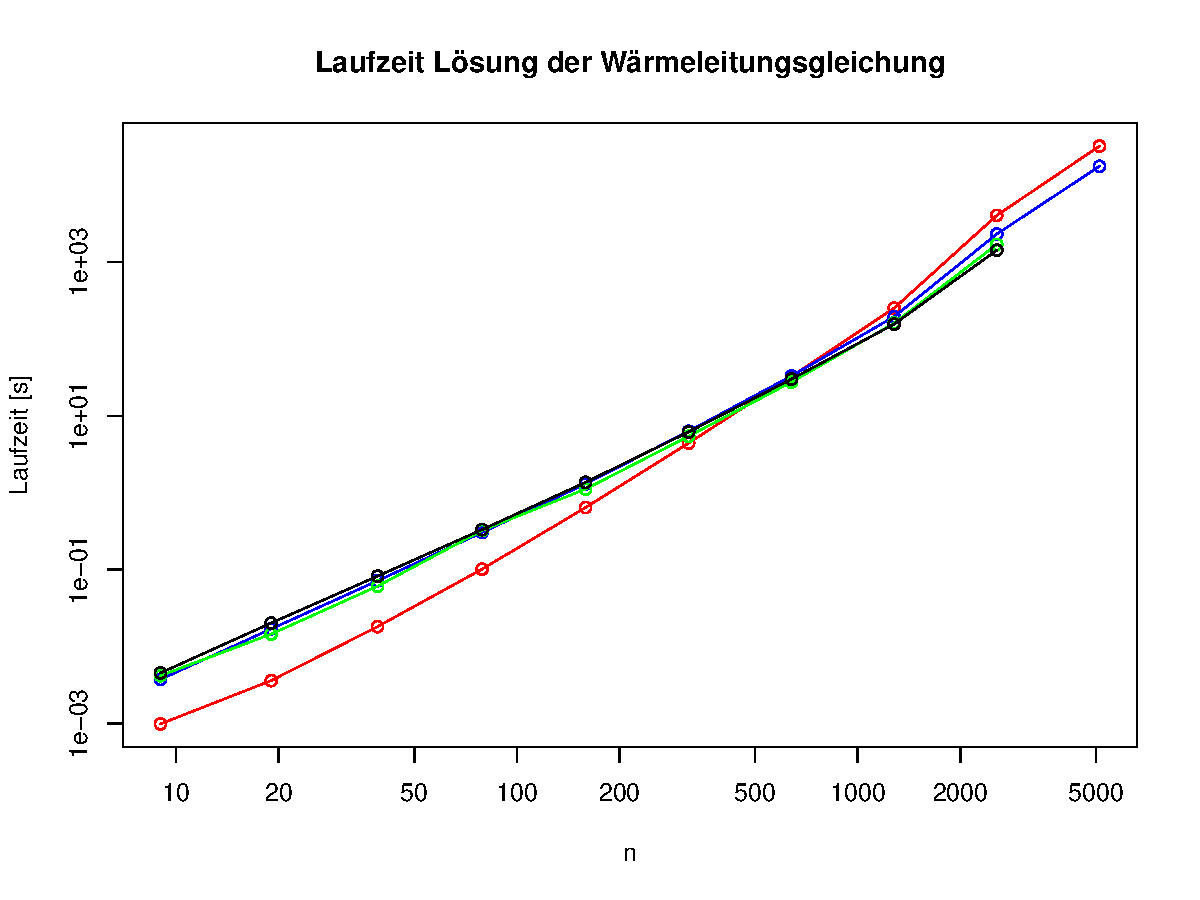
\includegraphics[width=\hsize]{heat/results-heat.pdf}
\end{center}
\caption{Laufzeit der mit OpenMP parallelisierten L"osung der
W"armeleitungsgleichung. Laufzeit mit einem einzelnen Thread ist rot
dargestellt.
\label{heat:laufzeit}}
\end{figure}

\subsection{OpenMPI}
Die Implementation mit OpenMP hat gezeigt, dass im eindimensionalen Fall
das Teilproblem zu klein ist, als dass die Parallelisierung des
Iterationsalgorithmus eine Laufzeitverbesserung ergeben k"onnte.
Das eindimensionale Problem wird also f"ur kleine $n$ am besten von einem
einzigen Prozessor gel"ost. 
Die Arbeit, die jeder Prozessor bis zum n"achsten Barrierepunkt
leistet, ist von der Gr"ossenordnung $O(n)$. 

Wenn eine parallele Implementation der L"osung der W"armeleitungsgleichung
eine bessere Laufzeit gegen"uber einer sequenziellen Implementation 
zeigen soll, dann muss die Menge der Arbeit, zwischen Barriere-Punkten
vergr"ossert werden.
Nur ein zwei- oder dreidimensionales W"armeleitungsproblem kann diese
Bedingung erf"ullen:
die Arbeit zwischen Barrierepunkten w"achst dann mit $O(n^2)$ bzw.~$O(n^3)$.

Die zweidimensionale W"armeleitungsgleichung
\[
\frac{\partial u}{\partial t}
=
\frac{\partial^2 u}{\partial x^2}
+
\frac{\partial^2 u}{\partial y^2}
\]
kann analog zur eindimensionalen W"armeleitungsgleichung diskretisiert
werden.
Die Funktion $u(t,x,y)$ wird ersetzt durch Variablen $u_{ijk}=u(ih_t,jh,kh)$.
Die zweiten partiellen Ableitungen nach $x$ und $y$ werden approximiert
werden (siehe auch Abbildung~\ref{heat:diskretisation2})
\begin{align*}
\frac{\partial^2u}{\partial x^2}
+
\frac{\partial^2u}{\partial y^2}
&
\simeq
\frac1{h^2}(
u_{i,j-1,k}-2u_{ijk}+u_{i,j+1,k}
)
+
\frac1{h^2}(
u_{i,j,k-1}-2u_{ijk}+u_{i,j,k+1}
)
\\
&=\frac1{h^2}(
u_{i,j-1,k}
+
u_{i,j,k-1}
+
u_{i,j+1,k}
+
u_{i,j,k+1}
-
4u_{ijk}
)
\end{align*}
F"ur diesen Operator wurde bereits fr"uher die Matrix $A$ in
(\ref{algorithm:laplace}) gefunden, die wir in "Ubereinstimmung mit
(\ref{heat:zerlegung}) wieder mit $N$ bezeichnen.
Dann wird die Iterationsformel wieder die gleiche Form haben wie
(\ref{heat:iteration}).
\begin{figure}
\begin{center}
\includegraphics[width=0.70\hsize]{heat/heat-2.pdf}
\end{center}
\caption{Approximation f"ur den Laplace-Operator $\Delta u$ im Punkt $(i,j)$
\label{heat:diskretisation2}}
\end{figure}

\begin{satz}
Das Iterationsverfahren (\ref{heat:iteration}) f"ur die zweidimensionale
W"armeleitungsgleichung konvergiert, wenn 
\begin{align*}
8\frac{h_t}{2h_x^2}&<1
&&\Leftrightarrow
&
h_t&<\frac{h_x^2}{4}.
\end{align*}
\end{satz}

\begin{figure}
\begin{center}
\includegraphics[width=0.8\hsize]{heat/heat-3.pdf}
\end{center}
\caption{Unterteilung des Definitionsbereiches in Teilbereiche (grau)
f"ur jeden OpenMPI Rang $r$, $0\le r<n_xn_y$.
Die d"unn ausgezogenen Rechtecke beinhalten Werte, die vor jedem 
Iterationsschritt ausgetauscht werden m"ussen.
\label{heat:domainpartition}}
\end{figure}

Zur Parallelisierung und Verteilung auf verschiedene Prozesse kann
der Definitionsbereich in $n_x$ Rechtecke in horizontaler Richtung
und $n_y$ Rechtecke in vertikaler Richtung zerlegt werden
(Abbildung~\ref{heat:domainpartition}).
Alle Teilrechtecke haben jeweils ungef"ahr die gleiche Gr"osse.
F"ur jedes Teilrechteck ist ein eigner OpenMPI Prozess zust"andig.

F"ur die Durchf"uhrung des Iterationsschrittes werden entlang des Randes
eines Teilrechtecks jeweils
die Variablen von den R"andern der Nachbarrechtecke ben"otigt.
Nach jedem Iterationsschritt m"ussen diese Werte zwischen den einzelnen
Prozessen ausgetauscht werden.
Beim Austausch fliessen die Daten in beiden Richtungen. Die Funktion
\verb+MPI_Send+ blockiert, bis die Daten im Zielprozess angekommen sind.
Daher wurde in der Implementation die Funktion \verb+MPI_Isend+ verwendet,
welche sofort zur"uckkommt. Alle Prozesse kopieren daher ihre Randdaten in
einen Sende-Puffer, und "ubermitteln ihn mit \verb+MPI_Isend+.
Danach k"onnen alle Prozesse die Rand-Daten in beliebiger Reihenfolge
empfangen. Wenn die Empfangs-Funktionen (\verb+MPI_Recv+) abgeschlossen sind,
dann sind auch die Sende-Operationen fertig.

Abbildung \ref{heat:threadzahl} zeigt die Abh"angigkeit der Laufzeit von der
Threadzahl f"ur ein Problem der Gr"osse $n=2560 \times 1440=3686400$.
F"ur einen einzelnen Iterationsschritt, also zwischen zwei Austauschschritten
f"ur die Randwerte m"ussen bei 4 Prozessen in jedem Prozess fast eine Million
Variablen neu berechnet werden, was mindestens 6 Rechenoperationen erfordert.
Damit ist sichergestellt, dass die reine Rechenzeit in den Iterationsschritten
die Gesamtzeit dominiert, was sich auch in der guten Skalierung bis
zur Gesamtzahl der Prozesse zeigt.

\begin{figure}
\begin{center}
\includegraphics[width=\hsize]{heat/results-heat-threads.pdf}
\end{center}
\caption{Laufzeit der mit OpenMPI parallelisierten L"osung der
W"armeleitungsgleichung in Abh"angigkeit von der Prozesszahl.
Mehr als vier Prozesse gegen auf der verwendeten 4-Prozessor-Maschine
keine verbesserte Laufzeit.
\label{heat:threadzahl}}
\end{figure}


